\documentclass[12pt]{tesis-filkom}

\title{Title and Description of The Document as a Template for the Thesis at Filkom Judulnya Sedikit Lebih Panjang}
\titleen{Judul Tesis dalam Bahasa Inggris}

\nama{Sunama Mahasiswa}
\nim{21234918239823}

\prodi{Magister Ilmu Komputer}
\departemen{Teknik Informatika}
\fakultas{Fakultas Ilmu Komputer}
\universitas{Universitas Brawijaya}
\tahun{2023}

\tanggalujian{4 September 2022}
\pembimbingsatu{Djoko Bimbing Satu, Ph.D}
\nikpembimbingsatu{NIP 123456789}

% kalau pembimbing tunggal
\pembimbingdua{}
\nikpembimbingdua{}

% kalau ada pembimbing dua
% enable dua baris command berikut ini:
\pembimbingdua{Dr. dr. Djoki Bimbing Dua, Dr.Sc}
\nikpembimbingdua{NIK 983298344}

% Jika ini adalah tesis (bukan proposal tesis)
% enable command \istesis berikut ini:
% \istesis

% Jika ini adalah naskah akhir
% enable dua baris command berikut ini:
\kadep{Dr.Phil Djoku Kadep, S.Kom., M.Dcs, Ph.D}
\nipkadep{NIP 001923189283398233}

\kotapernyataan{Malang}
\tanggalpernyataan{1 Januari 2015}







\begin{document}



\maketitle
\addtocontents{toc}{\vspace{5mm}}
\pagenumbering{roman}
\setcounter{page}{0}
\lembarpengesahan
\pernyataanorisinalitas{meterai}

\setstretch{1.05}
\setlength{\parskip}{0.25em}

% \pernyataanorisinalitas{}
\newpage
\centering{
  \MakeUppercase{
    \bfseries\LARGE{
      Kata Pengantar \\
    }
  }
}
\addcontentsline{toc}{section}{\MakeUppercase{Kata Pengantar}}
\vspace{10mm}
\normalsize
\justifying

Bagian ini memuat pernyataan resmi untuk menyampaikan rasa terima kasih penulis kepada berbagai pihak yang telah membantu penyelesaian tesis ini. 
Nama-nama penerima ucapan terima kasih sebaiknya dituliskan lengkap, termasuk gelar akademik, dan pihak-pihak yang tidak terkait dihindari untuk dituliskan. 
Bahasa yang digunakan seharusnya mengikuti kaidah bahasa Indonesia yang baku. 
Prakata boleh diakhiri dengan paragraf yang menyatakan bahwa penulis menerima kritik dan saran untuk pengembangan penelitian selanjutnya. 
Terakhir, prakata ditutup dengan mencantumkan kota dan tanggal penulisan prakata, lalu diikuti dengan kata "Penulis".

\vspace{10mm}
\hfill\begin{minipage}{\dimexpr\textwidth-9cm}
  Malang, 1 Januari 2015

  \vspace{10mm}
  Penulis \\
  email@domain.com
  \xdef\tpd{0}
\end{minipage}

% \addcontentsline{toc}{section}{Prakata}
% \addcontentsline{toc}{chapter}{List of Appendices}

\newpage
\centering{
  \bfseries\LARGE{
    ABSTRAK \\
  }
}
\addcontentsline{toc}{section}{\MakeUppercase{Abstrak}}
\vspace{10mm}
\normalsize
\justifying

% \noindent
% \textbf{\pnama, \ptitle}
% \textbf{
%   \noindent
%   \\Pembimbing: \ppembimbingsatu
%   \ifthenelse{\equal{\ppembimbingdua}{}}
%   {} {\phantom{ }dan \ppembimbingdua}}

% \vspace{5mm}

\indent
Bagian ini diisi dengan abstrak dalam Bahasa Indonesia. Abstrak adalah uraian singkat (umumnya 200-300 kata) yang merupakan intisari dari sebuah tesis. Abstrak membantu pembaca untuk mendapatkan gambaran secara cepat dan akurat tentang isi dari sebuah tesis. Melalui abstrak, pembaca juga dapat menentukan apakah akan membaca tesis lebih lanjut. Oleh karena itu, abstrak sebaiknya memberikan gambaran yang padat tetapi tetap jelas dan akurat tentang (1) apa dan mengapa penelitian dikerjakan: sedikit latar belakang, pertanyaan atau masalah penelitan, dan/atau tujuan penelitian; (2) bagaimana penelitian dikerjakan: rancangan penelitian dan metodologi/metode dasar yang digunakan dalam penelitian; (3) hasil penting yang diperoleh: temuan utama, karakteristik artefak, atau hasil evaluasi artefak yang dibangun; (4) hasil pembahasan dan kesimpulan: hasil dari analisis dan pembahasan temuan atau evaluasi artefak yang dibangun, yang dikaitkan dengan pertanyaan/tujuan penelitian.

Yang harus dihindari dalam sebuah abstrak diantaranya (1) penjelasan latar belakang yang terlalu panjang; (2) sitasi ke pustaka lainnya; (3) kalimat yang tidak lengkap; (3) singkatan, jargon, atau istilah yang membingungkan pembaca, kecuali telah dijelaskan dengan baik; (4) gambar atau tabel; (5) angka-angka yang terlalu banyak.

Di akhir abstrak ditampilkan beberapa kata kunci (normalnya 5-7) untuk membantu pembaca memposisikan isi tesis dengan area studi dan masalah penelitian. Kata kunci, beserta judul, nama penulis, dan abstrak biasanya dimasukkan dalam basis data perpustakaan. Kata kunci juga dapat diindeks dalam basis data sehingga dapat digunakan untuk proses pencarian tulisan ilmiah yang relevan. Oleh karena itu pemilihan kata kunci yang sesuai dengan area penelitian dan masalah penelitian cukup penting. Pemilihan kata kunci juga bisa didapatkan dari referensi yang dirujuk. 

\vspace{5mm}
\noindent
Kata kunci: abstrak, tesis, intisari, kata kunci, artefak

% \newpage
\centering{
  \bfseries\LARGE{
    ABSTRACT \\
  }
}
\addcontentsline{toc}{section}{Abstract}
\vspace{10mm}
\normalsize
\justifying

\noindent
\textbf{\pnama, \ptitleen}
\textbf{
  \noindent
  \\Supervisor: \ppembimbingsatu
  \ifthenelse{\equal{\ppembimbingdua}{}}
  {} {\phantom{ }and \ppembimbingdua}
}

\vspace{5mm}

\indent
Abstract in English.

\vspace{5mm}
\noindent
Keywords: abstrak, tesis, intisari, kata kunci, artefak


\addcontentsline{toc}{section}{\MakeUppercase{Daftar Isi}}
\tableofcontents
\listoffigures
\listoftables
\listofappendix

\newpage
\pagenumbering{arabic}
\setcounter{page}{1}


\chapter{Pendahuluan}

% \parindent=20pt
% \setlength{\parindent}{15pt}

Bagian utama tesis terdiri dari beberapa komponen atau bab yang tersusun dengan alur yang logis. Pendahuluan merupakan komponen/bab pertama yang harus menjelaskan apa yang dikerjakan dalam tesis dan mengapa ini dikerjakan. 

\section{Latar Belakang}

Bagian ini memuat penjelasan mengenai latar belakang munculnya ide sehingga penelitian ini dilakukan. Untuk mendapatkan masalah atau pertanyaan penelitian, penulis dapat melakukan inferensi dari fakta-fakta pendukung yang mungkin diperoleh dari literatur atau pengamatan. Penulis harus menjelaskan mengapa masalah yang diteliti dianggap penting dan menarik. Dapat juga diuraikan kedudukan masalah yang teliti ini dalam lingkup permasalahan yang lebih luas. Dalam menjelaskannya, penulis dapat menggunakan teknik piramida terbalik, yaitu memulai penjelasan dari yang lebih umum diikuti dengan yang semakin khusus dan terfokus pada masalah tertentu yang harus diselesaikan atau pertanyaan yang harus dijawab dalam penelitian ini. Dalam bagian ini dapat juga dimasukkan beberapa uraian singkat penelitian terdahulu yang dapat memperkuat alasan mengapa penelitian ini dilakukan. 

Untuk menjembatani antara latar belakang dan rumusan masalah, serta untuk membantu menjelaskan fokus penelitian, pada bagian akhir bagian ini dapat dituliskan sebuah pernyataan bahwa pengambilan topik tesis didasarkan pada alasan yang telah dikemukakan, misalnya "Berdasarkan kebutuhan akan akurasi dari pengukuran kadar gula dalam darah diperlukan suatu perangkat lunak bantu yang akan dikembangkan dalam tesis ini". Yang harus diperhatikan dalam penulisan latar belakang adalah adanya kesinambungan penjelasan antara latar belakang dengan bagian-bagian lain yang ditulis sesudahnya (rumusan masalah, tujuan, manfaat, dan batasan masalah).


\section{Rumusan Masalah}

Bagian ini memuat pertanyaan penelitian (research questions) yang dituliskan dalam kalimat tanya untuk mengarahkan penelitian, mendorong peneliti untuk menjawabnya, dan menarik minat pembaca. Pertanyaan penelitian umumnya memiliki ciri-ciri sebagai berikut:

\begin{enumerate}
  \item Jelas: disampaikan dengan struktur bahasa Indonesia yang baku, benar, dan mudah dipahami
  \item Relevan: sesuai dengan apa yang ingin diteliti dan menggunakan istilah-istilah yang sesuai dengan masalah serta konteks keilmuan terkait
  \item Fokus: terarah pada masalah yang ingin diselesaikan atau fenomena yang akan dijelaskan
  \item Menarik: diusahakan dapat mendorong keinginan peneliti untuk menjawab pertanyaan ini dan merangsang pembaca untuk mengikuti lebih jauh penelitian ini
  \item Dapat terjawab: dapat dijawab atau diukur hasilnya melaui proses penelitian sesuai dengan batasan waktu dan sumber daya yang ada 
\end{enumerate}


Berikut beberapa contoh pertanyaan penelitian yang sesuai dengan topik dan permasalahannya masing-masing:

\noindent\underline{Contoh 1:}

\noindent Topik: 

\begin{displayquote}
Pengembangan sistem pendukung keputusan seleksi penerimaan peserta didik baru menggunakan metode ELECTRE dan SAW (Studi kasus: SMA Brawijaya Smart School Kota Malang)
\end{displayquote}

Rangkuman masalah umum dari latar belakang (sudah tergambarkan dan tertuang dalam latar belakang dan tidak perlu dituliskan dalam subbab atau seksi tersendiri):

\begin{displayquote}
SMA BSS Malang memiliki kesulitan dalam proses seleksi penerimaan peserta didik baru berdasarkan keminatan masing-masing dengan mekanisme yang masih manual. Metode ELECTRE dan SAW dapat dimanfaatkan untuk mengolah data calon peserta didik dalam menentukan rekomendasi peserta didik baru yang diterima dalam kelompok peminatan tertentu.
\end{displayquote}

\noindent Pertanyaan penelitian:

\begin{enumerate}
  \item Bagaimanakah rancangan algoritme yang menggunakan metode ELECTRE dan SAW dalam sistem pendukung keputusan untuk seleksi penerimaan peserta didik baru SMA BSS Malang? 
  \item Bagaimanakah tingkat akurasi sistem pendukung keputusan Seleksi Penerimaan Peserta Didik Baru SMA BSS Kota Malang menggunakan metode ELECTRE dan SAW tersebut?  
\end{enumerate}

\noindent \underline{Contoh 2:}

\noindent Topik: 

\begin{displayquote}
Pengembangan sistem perangkat lunak untuk administrasi pendidikan di Pondok Pesantren Nurul Huda Malang
\end{displayquote}

Rangkuman masalah dari latar belakang (sudah tergambarkan dan tertuang dalam latar belakang dan tidak perlu dituliskan dalam subbab atau seksi tersendiri):

\begin{displayquote}
Pondok Pesantren Nurul Huda Malang membutuhkan sebuah sistem perangkat lunak yang dapat membantu pelaksanaan proses-proses bisnis di dalamnya, khususnya dalam administrasi pendidikan. Beberapa masalah ditemukan dalam proses-proses bisnis tersebut. Masalah ini diharapkan dapat terselesaikan dengan bantuan sejumlah fungsi yang ditawarkan oleh sistem perangkat lunak ini.
\end{displayquote} 

\noindent Pertanyaan penelitian:
\begin{enumerate}
  \item Bagaimanakah hasil analisis dan spesifikasi persyaratan sistem perangkat lunak untuk administrasi pendidikan di Pondok Pesantren Nurul Huda Malang yang sesuai dengan kebutuhan organisasi tersebut? 
  \item Bagaimanakah rancangan sistem perangkat lunak yang sesuai dengan spesifikasi persyaratan sistem tersebut? 
  \item Bagaimanakah hasil implementasi sistem perangkat lunak yang sesuai dengan rancangan sistem tersebut?
  \item Bagaimanakah hasil pengujian sistem perangkat lunak untuk administrasi pendidikan di pondok pesantren tersebut?
\end{enumerate}

\noindent\underline{Contoh 3:}

\noindent Topik: 

\begin{displayquote}
  Optimasi deteksi marker pada NyARToolKit menggunakan metode Ransac
\end{displayquote}

Rangkuman masalah dari latar belakang (sudah tergambarkan dan tertuang dalam latar belakang dan tidak perlu dituliskan dalam subbab atau seksi tersendiri):

\begin{displayquote}
Pembacaan marker pada aplikasi berbasis Augmented reality (AR) menggunakan pustaka NyARToolKit 4.0.3 masih kurang optimal jika digunakan untuk membaca marker yang tidak ideal. Untuk mengatasi kondisi tersebut, dibutuhkan metode, seperti metode Ransac, untuk mengoptimalkan kinerja aplikasi AR dalam membaca marker yang tidak ideal.
\end{displayquote}

\noindent Pertanyaan penelitian:

\begin{enumerate}
  \item Bagaimanakah rancangan aplikasi yang dapat meningkatkan kinerja AR terhadap pengenalan marker tidak ideal dengan metode RANSAC?
  \item Bagaimanakah mengimplementasikan algoritma metode RANSAC pada pustaka NyARToolKit 4.0.3?
  \item Bagaimana pengaruh metode RANSAC terhadap peningkatan performa pendeteksian marker? 
\end{enumerate}

\noindent\underline{Contoh 4:}

\noindent Topik: 
\begin{displayquote}
  Pengujian usability desain tata letak papan ketik berbasis QWERTY untuk penulisan teks Arab (studi kasus: Intellark, Nonosoft Khot, dan Arabic Pad)
\end{displayquote}


Rangkuman masalah dari latar belakang (sudah tergambarkan dan tertuang dalam latar belakang dan tidak perlu dituliskan dalam subbab atau seksi tersendiri):

\begin{displayquote}
Intellark, Nonosoft Khot, dan Arabic Pad adalah desain tata letak papan ketik berbasis QWERTY untuk penulisan teks Arab yang memiliki karakter masing-masing. Sampai sejauh ini belum diketahui tingkat usability ketiga desain tersebut terhadap pengguna Indonesia, khususnya dalam aspek kecepatan pengetikan, tingkat kesalahan pengetikan, dan kemudahan untuk dipelajari.  
\end{displayquote}

\noindent Pertanyaan penelitian:
\begin{displayquote}
  Bagaimana perbandingan tingkat usability dari Intellark, Nonosoft Khot, dan Arabic Pad dalam menuliskan teks Arab untuk pengguna Indonesia, dalam aspek:
  \begin{enumerate}
    \item kecepatan pengetikan,
    \item tingkat kesalahan pengetikan, dan
    \item kemudahan untuk dipelajarinya?   
  \end{enumerate}
\end{displayquote}

\noindent\underline{Contoh 5:}

\noindent Topik:

\begin{displayquote}
  Pengaruh kepercayaan pelanggan terhadap tingkat retensi pelanggan di Gerai XXX
\end{displayquote}

\noindent Pertanyaan penelitian:

\begin{enumerate}
  \item Bagaimana hubungan kepercayaan pelanggan terhadap tingkat retensi pelanggan di Gerai XXX?
  \item Bagaimana pengaruh kepercayaan pelanggan terhadap tingkat retensi pelanggan di Gerai XXX?  
\end{enumerate}

\noindent Catatan: 

Ada yang berpendapat bahwa rumusan masalah berisi pernyataan masalah (problem statement) sebagai rangkuman dari masalah yang tertuang dalam latar belakang. Untuk menghindari kerancuan, dalam panduan tesis ini rumusan masalah diartikan sebagai pertanyaan penelitian (bukan pernyataan masalah) dengan defnisi, ciri-ciri, dan contoh tersebut sebelumnya. 

Jika terdapat hipotesis yang harus diuji, hipotesis dapat dituliskan pada seksi rumusan masalah ini dengan kalimat pernyataan yang sederhana, spesifik dan jelas, menyebutkan variabel-variabel yang diuji. Hipotesis dapat juga dituliskan dalam bagian terpisah "Rumusan hipotesis" dan diletakkan setelah rumusan masalah. Hipotesis merupakan dugaan atau jawaban sementara dari pertanyaan atau masalah penelitian yang masih harus dibuktikan kebenarannya dalam penelitian ini.

Contoh hipotesis untuk topik dan pertanyaan penelitian pada Contoh 5 sebelumnya:
\begin{enumerate}
  \item Terdapat hubungan positif antara kepercayaan pelanggan dan tingkat retensi pelanggan di Gerai XXX. 
  \item Terdapat pengaruh positif antara kepercayaan pelanggan dan tingkat retensi pelanggan di Gerai XXX.
\end{enumerate}

\section{Tujuan}

Bagian ini berisi tujuan yang ingin dicapai dari tesis ini. Tujuan yang ditulis harus dapat memberikan arah pada capaian penelitian. Tujuan ini dapat terdiri dari beberapa butir yang masing-masing harus dituliskan dalam kalimat pernyataan yang sederhana dan jelas, sesuai dengan masalah penelitian dan hasil yang ingin dicapai. 

Berikut ini beberapa contoh penulisan tujuan sesuai dengan contoh-contoh rumusan masalah pada seksi sebelumnya.

\noindent\underline{Contoh 1:}

\noindent Tujuan:
\begin{enumerate}
  \item Merancang algoritme untuk seleksi penerimaan penerimaan peserta didik baru SMA BSS Malang dengan metode ELECTRE dan SAW ke dalam sebuah sistem pendukung keputusan
  \item Menguji tingkat akurasi sistem pendukung keputusan Seleksi Penerimaan Peserta Didik Baru SMA BSS Kota Malang yang menggunakan metode ELECTRE dan SAW 
\end{enumerate}

\noindent\underline{Contoh 2:}

\noindent Tujuan:
\begin{enumerate}
  \item Menganalisis dan menyusun spesifikasi persyaratan sistem perangkat lunak untuk administrasi pendidikan di Pondok Pesantren Nurul Huda Malang
  \item Merancang sistem perangkat lunak sesuai persyaratan untuk sistem perangkat lunak tersebut
  \item Mengimplementasikan rancangan sistem perangkat lunak tersebut
  \item Menguji sistem perangkat lunak tersebut secara fungsional dan non-fungsional (sesuai kebutuhan/masalah yang difokuskan)
\end{enumerate}

\noindent\underline{Contoh 3:}

\noindent Tujuan:
\begin{enumerate}
  \item Merancang aplikasi yang dapat meningkat kinerja AR terhadap marker yang tidak ideal dengan metode RANSAC
  \item Mengimplementasikan algoritma metode RANSAC pada pustaka NyARToolKit 4.0.3
  \item Menilai pengaruh metode RANSAC terhadap peningkatan performa marker. 
\end{enumerate}

\noindent\underline{Contoh 4:}

\noindent Tujuan:

Mengevaluasi usability dan mengetahui perbandingan tingkat usability dari Intellark, Nonosoft Khot, dan Arabic Pad dalam menuliskan teks Arab untuk pengguna Indonesia, khususnya dalam aspek:
\begin{enumerate}
  \item kecepatan pengetikan,
  \item tingkat kesalahan pengetikan,
  \item dan kemudahan untuk dipelajarinya  
\end{enumerate}

\noindent\underline{Contoh 5:}

\noindent Tujuan:
\begin{enumerate}
  \item Mengetahui hubungan kepercayaan pelanggan terhadap tingkat retensi pelanggan di Gerai XXX.
  \item Mengetahui pengaruh kepercayaan pelanggan terhadap tingkat retensi pelanggan di Gerai XXX.
\end{enumerate}

Tujuan penelitian dapat juga dituliskan terdiri dari tujuan umum (aim) dan tujuan-tujuan khusus (objectives) yang mengelaborasi tujuan umumnya. Contohnya adalah:

\begin{displayquote}
  Tujuan umum:

  Mengembangkan aplikasi piranti bergerak eHalal untuk identifikasi produk halal MUI di supermarket 
  
  Tujuan khusus:
  \begin{enumerate}
    \item Mengidentifikasi persyaratan fungsional dan non fungsional aplikasi eHalal
    \item Merancang aplikasi eHalal dengan pemodelan berorientesi objek
    \item Mengimplementasikan aplikasi eHalal dengan teknologi berorientasi obyek
    \item Menguji aplikasi eHalal sesuai dengan persyaratan fungsional dan non fungsionalnya 
  \end{enumerate}
\end{displayquote}
  
Sebagai tambahan, jika sebuah penelitian dimaksudkan untuk menguji hipotesis, maka paling tidak salah satu tujuannya berhubungan dengan pengujian hipotesis tersebut.


\section{Manfaat}

Manfaat penelitian dapat diuraikan sebagai dampak atau konsekuensi positif penelitian terhadap ruang lingkup masalah yang lebih luas dan/atau terhadap para pemangku kepentingan (stakeholders) yang terlibat di dalamnya. Manfaat penelitian seharusnya tidak meliputi pernyataan "untuk memenuhi persyaratan mencapai gelar sarjana" di program studi yang bersangkutan karena ini merupakan persyaratan akademik dan administratif  institusi, tidak berhubungan dengan substansi penelitiannya.

\section{Batasan Masalah}

Bagian ini dapat dituliskan untuk membantu menjelaskan ruang lingkup masalah penelitian dengan menyatakan hal-hal yang menjadi batasan dan asumsi-asumsi yang digunakan untuk menyelesaikan masalah yang sudah dirumuskan. 

Batasan-batasan yang sangat teknis dan tidak langsung berhubungan dengan fokus masalahnya, jika tetap diperlukan, sebaiknya diletakkan di bab lain yang lebih relevan. Sebagai contoh, untuk meneliti implementasi algoritma tertentu ke dalam sebuah kasus dengan fokus akurasi algoritme, jenis aplikasi editor untuk penyusunan kode program tidak perlu dituliskan di batasan masalah, tetapi lebih tepat di bab metodologi atau implementasi.   

Bagian batasan masalah ini dapat dihilangkan jika ruang lingkup masalah yang diuraikan dan direfleksikan melalui latar belakang, rumusan masalah, dan tujuan penelitian sudah cukup jelas.

\section{Sistematika Pembahasan}

Bagian ini berisi struktur tesis ini mulai Bab Pendahuluan sampai Bab Penutup dan detesis singkat dari masing-masing bab. Diharapkan bagian ini dapat membantu pembaca dalam memahami sistematika pembahasan isi dalam tesis ini. 
\newpage
\chapter{Landasan Kepustakaan}

Landasan kepustakaan berisi uraian dan pembahasan tentang teori, konsep, model, metode, atau sistem dari pustaka ilmiah, yang berkaitan dengan tema, masalah, atau pertanyaan penelitian. Dalam landasan kepustakaan terdapat landasan teori dari berbagai sumber pustaka yang terkait dengan teori dan metode yang digunakan dalam penelitian. Jika dibutuhkan sesuai dengan karakteristik penelitiannya dan syarat kecukupan khusus keminatan tertentu, bisa juga terdapat kajian pustaka yang menjelaskan secara umum penelitian-penelitian terdahulu yang berhubungan dengan topik tesis dan menunjukkan persamaan dan perbedaan tesis tersebut terhadap penelitian terdahulu yang dituliskan. 

\section{Subbab Dua Satu}

Isi landasan kepustakaan bukanlah sekedar salinan dari sumber pustaka, tetapi merupakan ringkasan, sintesis, atau kombinasi dari keduanya, terhadap informasi dari sumber pustaka. Ringkasan adalah uraian singkat dari hal-hal yang relevan dari sumber pustaka (Brown, 2005), sedangkan sintesis adalah reorganisasi atau penyusunan ulang berbagai informasi yang relevan tersebut sehingga secara keseluruhan membentuk kerangka teoritik dari penelitian (Richmod, 2005).

\subsection{Subbab Dua Satu Satu}

Dalam membuat ringkasan, informasi teoritik yang dipilih dari sumber pustaka haruslah yang benar-benar relevan dengan masalah penelitian. Oleh karena itu, peneliti harus kritis dalam menyeleksi informasi. Kemudian, untuk menjaga agar informasi yang dipilih memang berasal dari studi atau kajian ilmiah, disarankan menggunakan sumber-sumber pustaka ilmiah, seperti jurnal, prosiding konferensi atau seminar, tesis, disertasi, tesis, atau buku teks, dan dihindari sumber-sumber yang tidak jelas penulisnya atau kapasitas penulisnya. Jika informasi yang diambil dimaksudkan untuk pembahasan teori, konsep, atau metode terkini, maka sebaiknya sumber yang digunakan adalah yang semutakhir mungkin.

Menurut Berndtsson et al. (2008), dalam melakukan sintesis, informasi teoritik sebaiknya dijelaskan mulai dari informasi yang lebih umum dan secara bertahap menuju ke yang lebih khusus. Penulis juga seharusnya menjelaskan aspek-aspek mana dari informasi teoritik tersebut yang langsung berhubungan atau menjadi dasar dari masalah penelitian, serta bagaimana aspek tersebut berhubungan dengan masalah penelitian (Rumbaugh et al., 2005; Brodjonegoro, 2009a; Sommerville, 2011).

\subsection{Subbab Dua Satu Dua}

Ketika harus mengacu informasi dari sumber pustaka, penulis wajib memberikan apresiasi kepada penulis pustaka tersebut dengan cara menuliskan identitas pustaka tersebut beserta penulisnya dalam Daftar Pustaka dan mereferensi informasi tersebut dari badan tulisan dengan cara yang tepat.

Dalam berbagai laporan atau artikel ilmiah, landasan kepustakaan atau tinjauan kepustakaan dapat menjadi sebuah bab sendiri atau isinya menjadi bagian dari satu atau lebih bab yang lain. Selain itu, judul bab/subbab yang dipakai juga bervariasi, diantaranya adalah yang bersifat tematik. Oleh karena itu, jika diperlukan, judul bab Landasan Kepustakaan dalam tesis juga dapat digantikan dengan judul lain yang tematik dan deskriptif terhadap isi dari bab tersebut.

\section{Subbab Dua Dua}

Penulisan persamaan, tabel, gambar, dan symbol-simbol memiliki aturan khusus seperti yang dijelaskan dalam subbab-subbab berikut.

\subsection{Tentang Persamaan}

Setiap   persamaan   yang   digunakan   harus   diberi   nomor   berurutan  berdasar bab dan urutan munculnya persamaan. Huruf pertama suatu persamaan dimulai setelah 10 ketikan spasi dari batas kiri. Nomor persamaan ditulis di kanan persamaan dan ditempatkan pada batas kanan halaman dalam tanda kurung. 
Bilangan pertama menunjukkkan bab letak persamaan tersebut dan bilangan kedua yang dipisahkan tanda hubung merupakan nomor urutan persamaan dalam bab tersebut. 

Contoh inline equation, persamaan yang dituliskan langsung dalam baris kalimat. The well known Pythagorean theorem $x^2 + y^2 = z^2$ was proved to be invalid for other exponents. 
Meaning the next equation has no integer solutions:

\begin{equation}
  \label{eq:pythagorean}
  x^n + y^n = z^n
\end{equation}

Ketika persamaan ini diacu dari dalam teks maka dapat dituliskan sebagai Persamaan \ref{eq:pythagorean}.

\noindent Contoh penulisan pecahan:

\begin{equation}
  \binom{n}{k} = \frac{n!}{k!(n-k)!}
\end{equation}

\noindent Contoh penulisan limit:

\begin{equation}
  \lim_{h \to 0 } \frac{f(x+h)-f(x)}{h}
\end{equation}

\noindent Contoh penulisan dengan alignment:
\begin{align*}
  x&=y           &  w &=z              &  a&=b+c\\
  2x&=-y         &  3w&=\frac{1}{2}z   &  a&=b\\
  -4 + 5x&=2+y   &  w+2&=-1+w          &  ab&=cb \eqnumber \label{eqn:4}
\end{align*}

\noindent Penggunaan alignment yang menyertakan nomor persamaan:
\begin{align*}
  4x + 2y^2 = z \\
  a + b = c \eqnumber \label{eqn:1}
\end{align*}
 
\noindent Dengan grouping:
\begin{gather*} 
  2x - 5y =  8 \\ 
  3x^2 + 9y =  3a + c \label{eqn:2}
\end{gather*}

\noindent Menuliskan persamaan kompleks:
\begin{align*}
  S(\omega) 
  &= \frac{\alpha g^2}{\omega^5} e^{[ -0.74\bigl\{\frac{\omega U_\omega 19.5}{g}\bigr\}^{\!-4}\,]} \\
  &= \frac{\alpha g^2}{\omega^5} \exp\Bigl[ -0.74\Bigl\{\frac{\omega U_\omega 19.5}{g}\Bigr\}^{\!-4}\,\Bigr] \eqnumber \label{eqn}
\end{align*}

\subsection{Subbab Dua Dua Dua tentang Tabel}

Tabel berguna untuk menyajikan informasi yang detil dalam jumlah banyak. Setiap tabel memiliki nomor urut dan judul yang diletakkan di atas tabel. Nomor urut tabel terdiri atas nomor bab dan nomor urut kemunculan tabel itu dalam bab yang bersangkutan. Kedua nomor ini dipisahkan dengan titik. Penulisan nomornya serupa dengan penulisan nomor persamaan. Antara nomor tabel dan judul tabel dipisahkan oleh satu ketikan spasi. Judul tabel ditulis secara ringkas dan jelas, diawali dengan huruf kapital, diikuti dengan huruf kecil, tanpa diakhiri tanda titik, dan ditulis tebal (bold). Penulisan kata "Tabel" dalam naskah yang disertai dengan nomor tabel harus diawali dengan huruf kapital seperti pada contoh berikut: 

\begin{table}
  \caption{Pembentukan bilangan random untuk Indeks Masa Tubuh (IMT)}
  \centering
  \renewcommand{\arraystretch}{1.2}
  \begin{tabular}[ht]{clc}
    \hline
    No & Keanggotaan IMT & Rentang Nilai \\
    \hline
    1 & Sangat Kurus & 0.0 - 19.0 \\
    2 & Kurus & 15.0 - 20.0 \\
    3 & Normal & 17.0 - 27.0 \\
    4 & Gemuk & 23.0 - 29.0 \\
    5 & Obesitas & 25.0 - 50.0 \\
    \hline
  \end{tabular}
\end{table}

Judul tabel harus berada dalam satu halaman dengan tabelnya. Selain itu, sebuah tabel sebaiknya diusahakan untuk termuat dalam satu halaman, tidak terpenggal ke dalam lebih dari satu halaman. Untuk menghindari pemenggalan tabel, ukuran huruf dan spasi kata-kata dalam tabel dapat diperkecil tetapi harus tetap terbaca. 

Jika terpaksa dipenggal, tabel yang sama pada halaman berikutnya harus tetap diberi identitas di atasnya. Identitas ini terdiri dari kata "Tabel", no tabel, judul tabel (opsional) dan kata "(lanjutan)", misalnya:

Tabel 2.1 (lanjutan)  

atau

Tabel 2.2 Judul tabel (lanjutan)

Judul setiap kolom juga tetap harus dituliskan pada penggalan tabel di halaman berikutnya. Fitur yang relevan dalam program pengolah kata dapat digunakan untuk menjaga konsistensi ini. 

Contoh tabel yang terpaksa harus terpenggal dapat dilihat pada Tabel 2.2.

% \begin{table}
  % \renewcommand{\arraystretch}{1.2}
  \begin{longtable}{cl}
    
    \caption{Contoh tabel 2} \\
    % \renewcommand{\arraystretch}{1.2}
    % \begin{longtable}[h]{cl}
      \hline
      No & Nama Universitas di Indonesia \\
      \hline
      \endfirsthead
      \caption{Contoh tabel 2 (lanjutan)} \\
      \hline
      No & Nama Universitas di Indonesia \\
      \hline
      \endhead
      \hline
      \endfoot
      1 & Universitas 1 \\
      2 & Universitas 2 \\
      3 & Universitas 3 \\
      4 & Universitas 4 \\
      5 & Universitas 5 \\
      6 & Universitas 6 \\
      7 & Universitas 7 \\
      8 & Universitas 8 \\
      9 & Universitas 9 \\
      10 & Universitas 10 \\
      11 & Universitas 11 \\
      12 & Universitas 12 \\
      13 & Universitas 13 \\
      14 & Universitas 14 \\
      15 & Universitas 15 \\
      16 & Universitas 16 \\
      17 & Universitas 17 \\
      18 & Universitas 18 \\
      19 & Universitas 19 \\
      20 & Universitas 20 \\
      21 & Universitas 21 \\
      22 & Universitas 22 \\
      23 & Universitas 23 \\
      24 & Universitas 24 \\
      25 & Universitas 25 \\
      26 & Universitas 26 \\
      27 & Universitas 27 \\
      28 & Universitas 28 \\
      29 & Universitas 29 \\
      30 & Universitas 30 \\
      31 & Universitas 31 \\
      32 & Universitas 32 \\
      33 & Universitas 33 \\
      34 & Universitas 34 \\
      35 & Universitas 35 \\
      36 & Universitas 36 \\
      37 & Universitas 37 \\
      38 & Universitas 38 \\
      39 & Universitas 39 \\
      40 & Universitas 40 \\
      41 & Universitas 41 \\
      42 & Universitas 42 \\
      43 & Universitas 43 \\
      \hline
  \end{longtable}
% \end{table}

Jika sebuah tabel harus disajikan dalam bentuk landscape, maka bagian atas tabel harus diletakkan di sebelah kiri. Dalam hal ini nomor halaman harus tetap di tengah bawah.   

Jika sebuah tabel berasal dari sumber pustaka lainnya, maka sumber tersebut harus dituliskan sebagai referensi dalam daftar referensi dan sitasi terhadap referensi itu dituliskan di bawah tabel. Penjelasan lebih lanjut tentang sitasi gambar beserta contohnya dapat dilihat pada buku panduan. 

Sebuah tabel tidak berdiri sendiri tanpa teks yang merujuknya. Tabel dapat menggambarkan data yang disebutkan dalam teks atau sebaliknya teks dapat menjelaskan bagaimana data dalam tabel dilihat dan dianalisis. Tabel yang berada pada lampiran juga tetap harus dirujuk dari dalam bagian utama.

\subsection{Gambar}

Gambar dalam tesis dapat meliputi diagram, grafik, peta, foto, dan sebagainya. Sebagaimana tabel, setiap gambar memiliki nomor urut dan judul. Tetapi berbeda dengan tabel, nomor urut dan judul gambar diletakkan di bawah gambar. Nomor urut gambar terdiri atas nomor bab dan nomor urut kemunculan gambar tersebut dalam bab yang bersangkutan. Kedua nomor ini dipisahkan dengan titik. Penulisan nomornya serupa dengan penulisan nomor tabel. Antara nomor gambar dan judul gambar dipisahkan oleh satu ketikan spasi. Judul gambar ditulis secara ringkas dan jelas, diawali dengan huruf kapital, diikuti dengan huruf kecil, tanpa diakhiri tanda titik, dan ditulis tebal (bold). Penulisan kata "Gambar" dalam naskah yang disertai dengan nomor gambar harus diawali dengan huruf kapital seperti pada Gambar  2.1 berikut. 

\begin{figure}[ht]
  \centering
  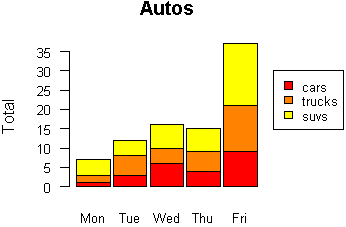
\includegraphics[width=.5\textwidth]{babs/images/bar_script4.png}
  \caption{Pengaruh nilai K terhadap akurasi}
  \label{fig:pengaruh}
\end{figure}


Judul tabel harus berada dalam satu halaman dengan tabelnya. Fitur yang relevan dalam program pengolah kata dapat digunakan untuk menjaga konsistensi ini.

Jika sebuah gambar harus disajikan dalam bentuk landscape, maka bagian atas gambar harus diletakkan di sebelah kiri. Dalam hal ini nomor halaman harus tetap berada di tengah bawah.   

Jika sebuah gambar berasal dari sumber pustaka lainnya, maka sumber tersebut harus dituliskan sebagai referensi dalam daftar referensi dan sitasi terhadap referensi itu dituliskan di bawah gambar. Penjelasan tentang sitasi gambar beserta contohnya dapat dilihat pada buku panduan tesis. 

Gambar berwarna sebaiknya dicetak berwarna atau diatur dengan pewarnaan yang kontras. Gambar yang dikutip dari sumber lain atau hasil pemindaian (scan) hendaknya diperhatikan tingkat resolusi dan ketajamannya.  

Sebuah gambar tidak berdiri sendiri tanpa teks yang merujuknya. Gambar dapat mengilustrasikan apa yang disebutkan dalam teks atau sebaliknya teks dapat menjelaskan apa yang berada dalam gambar. Gambar yang berada pada lampiran juga tetap harus dirujuk dari teks dalam bagian utama.

\subsection{Lambang, Satuan, dan Singkatan}

Penulisan lambang atau simbol sebaiknya menggunakan fasilitas simbol atau jenis huruf Symbol yang ada pada program komputer pengolah kata untuk membedakannya dengan huruf biasa. Sebagai contoh untuk tanda perkalian tidak menggunakan huruf x tetapi "$\times$" dari symbol. Untuk rumus matematika diusahakan ditulis dalam satu baris. Bila hal ini tidak memungkinkan maka harus diatur sedemikian rupa agar mudah dimengerti.
Satuan dan singkatan yang digunakan adalah yang lazim dipakai dalam disiplin ilmu terkait, misalnya 25\degree C; 10 ppm; H\textsubscript{2}O; dan sebagainya. Superscript dan subscript sebaiknya digunakan ketika diperlukan. Contoh penggunaan persamaan yang menggunakan superscript dan subscript:

\begin{equation}
  x_a^b = y_x
\end{equation}

\noindent atau contoh lainnya:

\begin{equation}
  \sum_{i=1}^{\infty} \frac{1}{n^s} 
= \prod_p \frac{1}{1 - p^{-s}}
  \label{persamaan:sigma}
\end{equation}

Sedangkan contoh penulisan subscript dan superscript dalam kalimat inline adalah seperti ini: in\textsubscript{bawah} dan out\textsuperscript{atas}. Namun jika yang dituliskan adalah sebuah persamaan matematika yang dituliskan secara inline: $x_y$ atau $x^y$. Berbeda dengan apa yang diperlihatkan dalam Persamaan \ref{persamaan:sigma}.

\subsection{Subbab Dua Dua Satu Tentang Sitasi Tabel dan Gambar}

Tabel atau gambar yang direproduksi dari sumber lain, baik itu disalin langsung secara keseluruhan, atau diadaptasi (misalnya, disesuaikan bentuk dan formatnya, atau ditambahkan keterngan legenda dengan tidak mengubah arti), harus dibuatkan referensinya dalam daftar referensi dan sitasinya di bawah tabel atau gambar tersebut \citep{Bloggs1950}.

Contoh:

Referensi dalam daftar referensi:

\begin{displayquote}
  \bibentry{anggariawan:2014} 
\end{displayquote}

Namun sitasi yang dilakukan dengan menyebutkan nama author seperti yang dikatakan oleh \cite{Bloggs1950} dalam kalimat dapat dituliskan dengan cara seperti ini. Gunakan \verb_\cite_ dan bukan \verb_\citep_ seperti contoh di atas.

\begin{table}
  \centering
  \renewcommand{\arraystretch}{1.2}
  \caption{Pembentukan bilangan random untuk Indeks Masa Tubuh (IMT). Sitasi untuk tabel yang disalin langsung.}
  \begin{tabular}{clc}
    \hline
    No & Keanggotaan IMT & Rentang Nilai \\
    \hline
    1 & Sangat Kurus & 0.0 - 19.0 \\
    2 & Kurus & 15.0 - 20.0 \\
    3 & Normal & 17.0 - 27.0 \\
    4 & Gemuk & 23.0 - 29.0 \\
    5 & Obesitas & 25.0 - 50.0 \\
    \hline
    \multicolumn{2}{l}{\footnotesize{Sumber: \cite{anggariawan:2014}}} \\
    \label{tab:judulpanjangjuga}
  \end{tabular}
\end{table}




\begin{table}
  \centering
  \renewcommand{\arraystretch}{1.2}
  \caption{Pembentukan bilangan random untuk Indeks Masa Tubuh (IMT). Sitasi untuk tabel yang diadaptasi.}
  \begin{tabular}{clc}
    \hline
    No & Keanggotaan IMT & Rentang Nilai \\
    \hline
    1 & Sangat Kurus & 0.0 - 19.0 \\
    2 & Kurus & 15.0 - 20.0 \\
    3 & Normal & 17.0 - 27.0 \\
    4 & Gemuk & 23.0 - 29.0 \\
    5 & Obesitas & 25.0 - 50.0 \\
    \hline
    \multicolumn{3}{l}{\footnotesize{Sumber: Diadaptasi dari \cite{anggariawan:2014}}} \\
    \label{tab:judulpanjang}
  \end{tabular}
\end{table}

Jika tabel atau gambar adalah hasil perujukan sekunder, maka penulisan sitasi mengikuti aturan perujukan sekunder. Contohnya:
\begin{displayquote}
  Sumber: \cite{anggariawan:2014} disitasi dalam \cite{Bloggs1950}
\end{displayquote}

Penulisan istilah "Sumber" hanya digunakan jika tabel atau gambar berasal dari sumber lainnya sehingga perlu dilakukan sitasi. Jika tabel atau gambar adalah hasil karya penulis sendiri, tentu tidak diperlukan sitasi dan penulisan sumber.

\begin{table}
  \centering
  \renewcommand{\arraystretch}{1.2}
  \caption{Tabel Judul Pendek}
  \begin{tabular}{clc}
    \hline
    No & Keanggotaan IMT & Rentang Nilai \\
    \hline
    1 & Sangat Kurus & 0.0 - 19.0 \\
    2 & Kurus & 15.0 - 20.0 \\
    \hline
    \multicolumn{3}{l}{\footnotesize{Sumber: Diadaptasi dari \cite{anggariawan:2014}}} \\
  \end{tabular}
  \label{tab:judulpendek}
\end{table}

Tabel yang diberi judul cukup pendek akan secara otomatis dituliskan dengan rata tengah seperti yang diperlihatkan pada Tabel \ref{tab:judulpendek}. Sedangkan tabel yang judulnya panjang sehingga harus dituliskan lebih dari satu baris akan dituliskan secara rata kiri seperti pada Tabel \ref{tab:judulpanjang} dan Tabel \ref{tab:judulpanjangjuga}. 


\subsection{Subbab Dua Dua Dua}

Berikut ini adalah contoh penggunaan daftar beberapa pernyataan yang tersusun bernomor dan yang berindeks alfabetik:

\begin{enumerate}
  \item Aspek satu berkaitan dengan: 
  \begin{enumerate}[label=\alph*.]
    \item Aspek satu a
    \item Aspek satu b 
  \end{enumerate}
  \item Aspek dua berkaitan dengan: 
  \begin{enumerate}[label=\alph*.]
    \item Aspek dua a
    \item Aspek dua b
    \item Aspek dua c 
  \end{enumerate}
\end{enumerate}

Aspek-aspek tersebut bisa dijelaskan lebih lanjut sesuai tujuan dan kebutuhan. Penulisan di atas adalah sebuah contoh. 

\subsection{Kode Sumber}

Kode sumber (source code) dapat dituliskan dalam bagian utama atau lampiran tesis hanya jika benar-benar dibutuhkan untuk memperjelas solusi yang diusulkan. Penulisannya dibatasi hanya pada bagian-bagian yang terpenting, misalkan metode atau algoritme utama yang digunakan. Akan tetapi lebih disarankan untuk menggantinya dengan pseudocode atau notasi lainnya. Hal ini karena penulisan kode sumber yang berlebihan hanya mempertebal tesis tanpa memberikan nilai tambah. Selain itu, kode sumber tersebut sebenarnya termasuk properti intelektual penulis yang seharusnya dilindungi. 

Jika terpaksa harus dituliskan, kode sumber menggunakan tipe huruf Courier New berukuran 9 dan berspasi single. Kemudian, kode sumber dimasukkan ke dalam kolom ke-2 sebuah tabel yang dilengkapi dengan nomor baris di kolom ke-1. Contoh penulisan kode sumber adalah sebagai berikut: 

\noindent\textbf{\textit{Algoritme 1: Fungsi Iteratif}}
\begin{Verbatim}[numbers=left,xleftmargin=5mm,fontsize=\small]
public static void main(String[] args) {    
  int first = 10, second = 20;
  System.out.println(first + " " + second);

  // add two numbers
  int sum = first + second;
  System.out.println("The sum is: " + sum);
}
\end{Verbatim}

\noindent Without line numbering

\noindent\textbf{\textit{Algoritme 2: Fungsi Iteratif}}

\begin{Verbatim}[fontsize=\small]
public static void main(String[] args) {    
  int first = 10, second = 20;
  System.out.println(first + " " + second);

  // add two numbers
  int sum = first + second;
  System.out.println("The sum is: " + sum);
}
\end{Verbatim}
\newpage
\chapter{Metodologi Penelitian}

Makna dari metodologi penelitian dapat dilihat dari dua sudut pandang. Pertama, dari pandangan umum dia bisa berarti sebuah cara sistematik untuk menyelesaikan masalah penelitian. Dalam hal ini dia juga dapat merupakan kumpulan cara (metode) yang lebih spesifik dalam penyelesaian masalah. Kedua, metodologi penelitian dapat dipahami sebagai sebuah ilmu untuk mempelajari bagaimana sebuah penelitian dilakukan secara sistematik. Dalam ilmu ini kita mempelajari berbagai langkah yang umumnya digunakan oleh peneliti ketika mempelajari masalah penelitian beserta alasan-alasan logis di belakangnya. Oleh karena itu di dalam pembahasan metodologi penelitian, yang dibicarakan tidak hanya metode, teknik, atau langkah-langkah yang digunakan dalam sebuah penelitian tetapi juga logika di balik metode, teknik, atau langkah-langkah tersebut sesuai dengan konteks penelitiannya masing-masing. Dalam hal ini perlu dijelaskan mengapa sebuah metode atau teknik dipilih. 

\begin{figure}[ht]
  \centering
  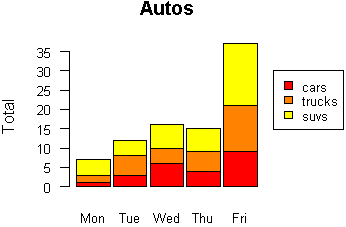
\includegraphics[width=.5\textwidth]{babs/images/bar_script4.png}
  \caption{Pengaruh nilai K terhadap akurasi}
  \label{fig:pengaruh2}
\end{figure}


\section{Subbab Tiga Satu}
Dari penjelasan di atas dapat dikatakan bahwa metodologi penelitian memiliki cakupan lebih luas daripada metode. Metode sendiri dapat diartikan sebagai cara, prosedur, atau teknik untuk menjalankan sebuah proses secara logis, terurut, dan sistematik. Metode/teknik dapat berupa metode/teknik untuk pengumpulan data, untuk analisis data, atau algoritme untuk pemecahan masalah penelitian. Terkadang metode dibedakan dari teknik dengan pemahaman bahwa teknik itu lebih khusus dan operasional daripada metode. Dalam panduan penulisan ini pemilihan istilah tersebut diserahkan kepada penulis dan pembimbingnya. Yang terpenting, apapun metode/teknik yang dipilih harus sesuai dengan sifat penelitian, masalah yang hendak diselesaikan, dan pertanyaan yang hendak dijawab. 

\subsection{Subbab Tiga Satu Satu}

Hal-hal yang perlu dijelaskan dalam metodologi penelitian adalah: 
\begin{enumerate}
  \item Tipe penelitian. Misalkan, nonimplementatif (deskriptif atau analitik) atau implementatif (pengembangan, perancangan, atau lainnya)
  \item Strategi dan rancangan penelitian 
  \begin{itemize}
    \item Strategi/metode secara umum. Misalnya, pembuatan artefak TI, studi kasus, survey, eksperimen, dan sebagainya. 
    \item Subjek atau partisipan penelitian. Siapa saja yang terlibat secara langsung dalam penelitian sebagai pelaku atau orang yang diambil datanya, serta bagaimana karakteristiknya yang dibutuhkan.
    \item Lokasi penelitian. Misalkan, di laboratorium atau studi lapangan di mana.
    \item Metode/teknik pengumpulan data. Misalnya, wawancara, observasi, kuisioner, studi dokumen.
    \item Metode/teknik analisis data dan pembahasan hasilnya. Misalnya, analisis kuantitatif secara statistik menggunakan uji t, analisis kualitatif terhadap teori A, B, dan sebagainya.
    \item Peralatan pendukung yang digunakan. Misalnya, spesifikasi piranti keras dan piranti lunak untuk menyusun kode sumber atau menguji sistem yang dibangun.
    \item Metode/teknik lainnya. Misalkan, jika strategi yang dipilih adalah pembangunan perangkat lunak, umumnya perlu dijelaskan model proses perangkat lunak yang digunakan. Sebagai catatan, Bab Metodologi Penelitian terfokus pada menjelaskan cara meneliti, sementara hasilnya dituliskan dalam bab-bab berikutnya. Oleh karena itu, dalam menjelaskan aktivitas dalam proses perangkat lunak, perlu dihindari dalam bab ini penjelasan daftar persyaratan/kebutuhan yang telah diidentifikasi, hasil perancangan, dan sebagainya. Contoh lainnya, untuk implementasi algoritma, perlu disebutkan dan dapat dideksripsikan secara singkat fungsi algoritme tersebut. Penjelasan yang lebih detil tentang algoritme tersebut dapat dimasukkan dalam bab lainnya, misalkan Bab Perancangan. 
  \end{itemize}
\end{enumerate}

Dalam mendetesiskan hal-hal di atas, penulis dapat menyusun subbab-subbab atau subbab-subbab beserta alur logikanya dengan pertimbangan sendiri di bawah supervisi pembimbing, berdasarkan relevansi dengan sifat penelitian dan aspek keterbacaan.

\subsection{Subbab Tiga Satu Dua}

Penomoran subbab disarankan tidak lebih dari 4 level (maksimal subbab X.X.X.X), tetapi sebaiknya hanya sampai 3 level. Kepala bab dan subbab tidak boleh mengandung widow atau orphan sehingga nampak menggantung atau terputus di bagian awal atau akhir sebuah halaman. Widow adalah sebuah paragraf dengan hanya satu baris pertama pada akhir halaman sedangkan sisanya berada pada halaman berikutnya. Orphan adalah baris terakhir dari satu paragraf yang tertulis pada awal suatu halaman sedangkan baris lainnya dari paragraf tersebut berada pada halaman sebelumnya.

\section{Subbab Tiga Dua}

Detesis dari subbab tiga dua, dan seterusnya.



\newpage
\chapter{Hasil}
 
Hasil berfungsi untuk melaporkan hasil pelaksanaan metode/teknik penelitian dan menyajikan data yang mendukung hasil tersebut. Penyajian data dan penjelasannya dilakukan secara terurut dan logis menggunakan teks dan ilustrasi lainnya (misalnya, tabel dan gambar). Urutan penjelasan dapat dilakukan secara kronologis berdasarkan urutan pelaksanaan metode atau berdasarkan tingkat kepentingan substansinya, dari yang lebih penting sampai ke yang proritasnya lebih rendah. 

\section{Subbab Dua Satu}

Sebelum menuliskan hasil ke dalam laporan, perlu dicermati dan ditentukan mana hasil yang relevan dan dapat digunakan untuk menjawab pertanyaan atau masalah penelitian.  Hasil inilah yang perlu dimasukkan terlepas dari apakah hasil ini positif (misalnya, mendukung kebenaran hipotesis) atau negatif (misalnya, menolak hipotesis). Selanjutnya, perlu diperhatikan bagaimana menyajikannya dengan cara terbaik, apakah dengan teks, tabel atau gambar. Tabel dan gambar (foto, gambar, grafik, diagram) sering digunakan untuk mempresentasikan data yang detil dan kaya, sementara teks digunakan untuk menarasikan temuan yang lebih umum dan menjelaskan bagian-bagian tertentu yang menjadi fokus dalam tabel dan gambar. 

\begin{table}[htbp]
  \centering
  \renewcommand{\arraystretch}{1.2}
  \caption{Tabel Judul Pendek di BAB 4}
  \begin{tabular}{clc}
    \hline
    No & Keanggotaan IMT & Rentang Nilai \\
    \hline
    1 & Sangat Kurus & 0.0 - 19.0 \\
    2 & Kurus & 15.0 - 20.0 \\
    \hline
    \multicolumn{3}{l}{\footnotesize{Sumber: Diadaptasi dari \cite{anggariawan:2014}}} \\
  \end{tabular}
  \label{tab:dibab4}
\end{table}


\section{Subbab Dua Dua}

Hasil dan pembahasan dapat diletakkan dengan kemungkinan berikut:
\begin{enumerate}
  \item	Dipisahkan secara fisik ke dalam bab-bab yang berbeda
  \item Dipisahkan secara fisik ke dalam dua atau lebih paragraf atau subbab yang berbeda tetapi dalam bab yang sama
  \item Dileburkan menjadi satu dalam paragraf, dijelaskan secara naratif-deskriptif, terdistribusi ke satu atau lebih bab yang ada
\end{enumerate}

\subsection{Subbab Empat Dua Satu}

Cara pertama atau kedua membantu pembaca yang ingin memisahkan observasi dan terjemahan dari observasi tersebut sehingga mereka dapat menilai kualitas dari masing-masing proses dengan lebih mudah. Kadang-kadang cara kedua lebih banyak dipilih daripada cara pertama jika data yang harus dipresentasikan yang cukup banyak dan laporan penelitian cukup panjang agar pembaca tidak perlu menunggu presentasi dari seluruh data selesai baru dapat membaca penerjemahannya. Cara pertama dan kedua ini banyak digunakan untuk penelitian yang bersifat kuantitatif, baik itu deskriptif, analitik, maupun implementatif.    

\subsection{Subbab Empat Dua Dua}

Cara ketiga biasanya digunakan jika data, analisis, dan penafsirannya sulit dipisahkan. Pemisahannya terkadang justru membuat laporan penelitian sulit dibaca. Hal ini dapat berlaku pada tipe penelitian yang bersifat kualitatif, baik itu deskriptif ataupun analitik/eksplanatori. 
Pada dasarnya peletakan dan jumlah bab untuk hasil dan pembahasan sebaiknya disesuaikan karakter penelitian masing-masing. Judul bab pun tidak harus secara eksplisit "Hasil" dan "Pembahasan" tetapi dapat digantikan dengan nama yang lebih deskpritif dan tematik. 

\section{Subbab Empat Tiga}

Contoh struktur tesis untuk implementatif pembangunan dan nonimplementatif dapat dilihat pada kedua subbab berikut. 

\subsection{Contoh Struktur Penelitian Implementatif Pengembangan}

Berikut ini adalah contoh bab-bab yang terdapat pada penelitian implementatif pengembangan sistem perangkat lunak. 
\begin{displayquote}
  Bab 1 Pendahuluan \\
  Bab 2 Landasan kepustakaan \\
  Bab 3 Metodologi penelitian \\
  Bab 4 Rekayasa persyaratan/kebutuhan \\ 
  Bab 5 Perancangan dan implementasi \\
  Bab 6 Pengujian \\
  Bab 7 Penutup \\
\end{displayquote}

Bab 1 sampai Bab 3 memuat informasi yang sesuai dengan panduan sebelumnya. Isi dari bab-bab berikutnya disesuaikan dengan syarat kecukupan tesis untuk tipe implementatif berdasarkan keminatan masing-masing, seperti yang terdapat pada panduan kecukupan tesis dan aturan khusus dari keminatan masing-masing. Di bawah ini adalah sebuah contoh saja: 

\begin{displayquote}
  Bab 4 Persyaratan:
  \begin{itemize}
    \item Pernyataan masalah yang lebih elaboratif/mendetail daripada yang di Pendahuluan.
    \item Identifikasi pemangku kepentingan (stakeholders) dan aktor (actors) sistem.
    \item Daftar terstruktur persyaratan/kebutuhan perangkat lunak, secara fungsional, data, dan nonfungsional
    \item Use cases, use case diagrams, use case specifications, dan sebagainya. 
  \end{itemize} 
  Bab 5 Perancangan dan implementasi:
  \begin{itemize}
    \item Rancangan arsitektur: detesis struktur dan setiap komponen utama
    \item Representasi data dalam model data dan basis data
    \item Detil implementasi dari fungsi-fungsi utama yang menjadi fokus
  \end{itemize}
  Bab 6 Pengujian dan evaluasi
  \begin{itemize}
    \item Strategi, rencana, kasus, dan data pengujian
    \item Ringkasan hasil pengujian perangkat lunak, termasuk data dan analisisnya (detilnya di Lampiran)
    \item Evaluasi hasil proyek secara keseluruhan, misalkan 
  \end{itemize}
  Bab 7 Penutup
  \begin{itemize}
    \item Ringkasan dari capaian proyek
    \item Saran pengembangan lebih lanjut
  \end{itemize}
\end{displayquote}

Pada contoh struktur ini "hasil" tersebar di beberapa bab mulai Bab 4 Persyaratan sampai Bab 6, sedangkan "pembahasan" secara keseluruhan terhadap masalah penelitian terdapat di Bab 6. Yang dimaksud dengan pengujian dalam Bab 6 terfokus pada pengujian persyaratan perangkat lunak, sedangkan evaluasi berfungsi sebagai "pembahasan" secara keseluruhan, yaitu menentukan apakah "hasil" sudah menjawab masalah penelitian yang dirumuskan pada Bab 1. 

Sebagai catatan, Bab 3 Metodologi Penelitian umumnya menjelaskan model proses perangkat lunak yang digunakan. Jika strategi untuk setiap aktivitasnya (analisis persyaratan, perancangan, dan seterusnya) sudah dijelaskan di Bab 3 ini juga, maka bab-bab lainnya yang berhubungan dengan aktivitas-aktivitas ini masing-masing langsung dapat menjelaskan hasil pelaksanaan metodenya. 

\subsection{Contoh Struktur Penelitian Nonimplementatif}

Berikut ini adalah contoh bab-bab yang terdapat pada penelitian nonimplementatif. 

\begin{displayquote}
  Bab 1 Pendahuluan \\
  Bab 2 Landasan kepustakaan \\
  Bab 3 Metodologi Penelitian \\
  Bab 4 Hasil \\
  Bab 5 Pembahasan \\
  Bab 6 Penutup
\end{displayquote}

Isi dari setiap bab dapat menyesuaikan dengan panduan yang telah dijelaskan sebelumnya. Jika diperlukan, Bab 4 dapat digabungkan dengan Bab 5, menjadi Hasil dan Pembahasan. 

Struktur dasar ini cukup universal sehingga dapat digunakan juga untuk tipe-tipe penelitian lainnya, khususnya jika belum ada struktur lain yang lebih tematik dan cocok untuk penelitian yang bersangkutan. Untuk lebih tepatnya, struktur penulisan menyesuaikan dengan studi keminatan serta saran dari dosen pembimbing masing-masing.

\newpage
\chapter{Pembahasan}

Pembahasan berfungsi untuk menerjemahkan makna dari hasil yang diperoleh untuk menjawab pertanyaan atau masalah penelitian. Fungsi lainnya adalah untuk menjelaskan pemahaman baru yang didapatkan dari hasil penelitian, yang diharapkan berguna dalam pengembangan keilmuan. Dalam penelitian tingkat lanjut, fungsi pembahasan yang kedua ini sangat penting karena dapat menunjukkan kontribusi penulis terhadap pengembangan keilmuan. Akan tetapi, dalam penelitian tingkat tesis, fungsi yang kedua ini dapat diterapkan secara terbatas karena pendidikan S1 tidak dituntut untuk pengembangan keilmuan secara substansial, tetapi cukup terhadap pemahaman personal dalam implementasi konsep atau teori. 

\section{Subbab Lima Satu}

Dalam menjawab masalah penelitian, penulis diminta untuk melakukan evaluasi kritis terhadap hasil yang diperoleh. Tergantung dari fokus penelitian, beberapa contoh pertanyaan kritis yang dapat dijawab adalah:
\begin{itemize}
  \item Seberapa jauh tujuan penelitian telah tercapai?
  \item Apakah aplikasi atau sistem yang dibangun sesuai dengan tujuannya?
  \item Apakah metode atau praktik perancangan dan implementasi yang baik telah dijalankan?
  \item Apakah teknologi implementasi yang tepat telah dipilih? Dan sebagainya. 
\end{itemize} 

\section{Subbab Lima Dua}

Dalam menjelaskan pemahaman baru yang didapatkan, penulis dapat mengubungkan hasil penelitian dengan pengetahuan teoritik atau penelitian sebelumnya yang telah dibahas. Kaitan antara hasil penelitian dan pengetahuan teoritik misalnya berupa:
\begin{itemize}
  \item pendapat tentang metode yang digunakan dari pustaka, apakah dapat digunakan dengan baik secara langsung, dengan penyesuaian, atau dengan batasan tertentu;
  \item konfirmasi tentang batasan dari metodologi yang digunakan sehingga dapat berpengaruh pada hasil;
  \item penjelasan tentang informasi penting pada penelitian lainnya yang membantu penulis untuk menerjemahkan data penelitian penulis;
  \item penjelasan tentang kemungkinan hasil dari penelitian lainnya yang dapat dikombinasikan dengan penelitian penulis untuk memberikan pengetahuan baru; dan sebagainya. 
\end{itemize}

\section{Subbab Lima Tiga}
Penulis dapat merefleksikan apa yang telah dipelajari selama melakukan penelitian, tetapi harus tetap terfokus dengan masalah penelitian ini dan tidak melebar ke masalah lainnya. Hal-hal yang berada di luar fokus peneltian tetapi penting dan menarik untuk diteliti dapat disarankan sebagai bahan penelitian berikutnya. Hal ini dapat dipertegas di bab Kesimpulan/ Penutup. 


\newpage
\chapter{Penutup}

Bagian ini memuat kesimpulan dan saran terhadap tesis. Kesimpulan dan saran disajikan secara terpisah, dengan penjelasan sebagai berikut: 

\section{Kesimpulan}

Kesimpulan merupakan pernyataan-pernyataan yang singkat, jelas, dan tepat tentang hasil penelitian yang diperoleh berdasarkan tujuannya. Bagian ini merupakan penegasan dari yang telah dijelaskan pada bagian Pembahasan dan tidak memuat informasi yang baru. Bagian ini juga mencerminkan jawaban dari rumusan masalah (pertanyaan penelitian).

\section{Saran}

Saran berisi pernyataan-pernyataan yang ringkas dan jelas tentang masalah-masalah atau hal-hal yang dapat dilakukan untuk mengembangkan penelitian ini lebih lanjut. Saran itu dapat diarahkan pada aspek metode, instrumen, populasi/sampel, dan sebagainya.



\renewcommand{\refname}{\centering\LARGE\MakeUppercase{Daftar Pustaka}}
\addcontentsline{toc}{section}{\MakeUppercase{Daftar Pustaka}}
\bibliography{referensi}
\bibliographystyle{apalike}

\newpage
\chapter*{\LARGE Lampiran}
\addcontentsline{toc}{section}{\MakeUppercase{Lampiran}}

\myappendix{Pertanyaan Wawancara} 
\label{appendix:a}
\lipsum[5]

\subappendix{Wawancara Group A} \lipsum[6]
\subappendix{Wawancara Group B} \lipsum[6]
\myappendix{Kuesioner Likert} \lipsum[7]
\subappendix{Likert 1} \lipsum[8]
\subappendix{Likert 2} \lipsum[8]



\end{document}